% Nejprve uvedeme tridu dokumentu s volbami
\documentclass[slovak,master,dept460,male,cpp,cpdeclaration]{diploma}
% Dalsi doplnujici baliky maker
\usepackage[autostyle=true,czech=quotes]{csquotes} % korektni sazba uvozovek, podpora pro balik biblatex
%\usepackage[backend=biber, style=iso-numeric, alldates=iso]{biblatex} % bibliografie
\usepackage{dcolumn} % sloupce tabulky s ciselnymi hodnotami
\usepackage{subfig} % makra pro "podobrazky" a "podtabulky"
\usepackage{verbatim}
\usepackage{cite}
\bibliographystyle{unsrt}
\nocite{*}
% Zadame pozadovane vstupy pro generovani titulnich stran.
\ThesisAuthor{Michal Falát}

\CzechThesisTitle{Analýza řidiče za pomocí sférických kamer}

\EnglishThesisTitle{Driver Analysis Using Spherical Cameras}

\SubmissionDate{1. apríla 2020}

% Pokud nechceme nikomu dekovat makro zapoznamkujeme.
\Thanks{Rád by som poďakoval môjmu vedúcemu práce Ing. Radovanovi Fusekovi za pomoc a ochotu pri vypracovaní diplomovej práce}

% Zadame cestu a jmeno souboru ci nekolika souboru s digitalizovanou podobou zadani prace.
% Pokud toto makro zapoznamkujeme sazi se stranka s upozornenim.
\ThesisAssignmentImagePath{Figures/Assignment1.jpg}
% \SlovakBachelorMaleAuthorDeclaration

% Zadame soubor s digitalizovanou podobou prohlaseni autora zaverecne prace.
% Pokud toto makro zapoznamkujeme sazi se cisty text prohlaseni.ss
% \AuthorDeclarationImageFile{Figures/AuthorDeclaration.jpg}


% Zadame soubor s digitalizovanou podobou souhlasu spolupracujici prav. nebo fyz. osoby.
% Pokud toto makro zapoznamkujeme sazi se cisty text souhlasu.
% \CooperatingPersonsDeclarationImageFile{Figures/CoopPersonDeclaration.jpg}

\CzechAbstract{Hlavnou témou diplomovej práce je rozpoznávanie a analýza vodiča v aute pomocou sférických kamier. Táto práca je rozdelená do viacerých samostatných častí. Prvá časť spočíva v samotnej detekcii ľudí a ich aktivít sférickou kamerou, hľadanie nedostatkov a nájdenie optimálnych parametrov pre čo najefektívnejšiu detekciu. Druhá časť je zameraná na porovnanie jednotlivych knižníc a metód, ktoré sa používaju na analýzu ľudského tela a tváre v obraze. Posledná časť je venovaná porovnaniu týchto metód s použitím reálnych dát zachytených sférickou kamerou a zhrnutie výsledkov. }

\CzechKeywords{Sférická kamera, detekcia obrazu, analýza ľudskej tváre, detekcia ľudí, vodič}

\EnglishAbstract{Main focus of this Diploma thesis is detection and analysis of driver in car with help of spherical cameras. This thesis is divided into few parts. The first part is about detection itself, detection of people by spherical cameras, research of disadvantages and finding optimal parameters for most efficnet detection. The second aprt is focused on comparision of libraries used for  human body and face detections. The last part is  about comparision of libraries with  real datas captured by  spherical camera and summary of results.  }

\EnglishKeywords{Spherical camera, image detection, analysis of human face, pedestrian detection, driver }

\AddAcronym{CPU}{Central processing unit}
\AddAcronym{FPS}{Frames per second}
\AddAcronym{GPU}{Graphical processing unit}
\AddAcronym{HOG}{Histogram oriented gradients}
\AddAcronym{OpenCV} {Open Source Computer Vision}
\AddAcronym{PX}{Pixel}



% Novy druh tabulkoveho sloupce, ve kterem jsou cisla zarovnana podle desetinne carkyss
\newcolumntype{d}[1]{D{,}{,}{#1}}


% Zacatek dokumentu
\begin{document}

% Nechame vysazet titulni strany.
\MakeTitlePages

% A nasleduje text zaverecne prace.
\section{Úvod}
\label{sec:Introduction}
V dnešnom modernom svete sú autá takmer každodennou súčasťou života ľudí. Mnohokrát sa ani nezamýšľame nad ich bezpečnosťou, ktorá je v prípade zrážky kľúčová. V súčasnosti nám pri jazde autom asistuje veľké množstvo systémov, ktoré zvyšujú bezpečnosť posádky, ale aj ostantých účastníkov cestnej premávky. Aj keď tieto systémy ešte stále nedokážu vodiča úplne nahradiť, dokážu mu výrazným spôsobom pomôcť napríklad v krízových situáciach. Výhodou takýchto systémov je ich rýchlejší reakčný čas oproti človeku. Takéto systémy spočívajú v použití rôznych snímačov alebo kamier, ktoré aktívne sledujú okolie ale aj interiér vozidla. Vďaka takýmto moderným technickým riešeniam je možné predísť rôznym  častokrát aj smrteľným dopravným nehodám. Výrobcovia áut sa čoraz častejšie snažia svoje systémy vylepšovať na čo najvyššiu možnú úroveň a poskytnúť tak vysoký level ochrany.\par Táto diplomová práca sa zameriava hlavne na problematiku analýzy vodiča pomocou detekcie obrazu zo sférickej (360-stupňovej) kamery. V diplomovej práci som sa venoval analýze videa z kamery umiestnenej v interiéri vozidla. Vhodným umiestnením kamery je možné získať obraz zpred auta, ale aj obraz vodiča sediaceho za volantom. V tejto práci som sa zameriaval na analýzu a spracovanie videa z interiéru vozidla na zachytenie ľudských aktivít vodiča. Aby som získal čo najväčšiu časť tela vodiča, je potrebné mať dostatočne veľký uhol záberu. Bežné kamery majú uhol záberu veľmi nízky, aby dokázal z malej vzdialenosti zachytiť celý snímaný objekt. Takýto problém sa naskytuje najpríklad aj v interiéri vozidla, kde je vzdialenoť kamery od snímaného objektu menej ako 1 meter, čo nemusí byť dostatočné na zosnímanie tela celého vodiča. Práve v takejto situácii je vhodné použiť širokouhlú prípadne sférickú kameru. Počas práce som mal k dispozicii viaceré kamery, s ktorými som zhotovol niekoľko desiatok videí v rôznych situáciach. Z takýchto videi som dokázal analyzovať a zistiť mnoho užitočných informácii, ktore sú spracované v tejto diplomovej práci. Tieto informácie som zbieral nahrávaním videa sférickymi kamerami za rôznych svetelnych  podmienok a pozicií vodiča. V tejto práci sú taktiež spomenuté problémy takejto analýzy, riešenia vzniknutých problémov, ale aj zhrnutie celkovej problematiky sledovania vodiča vo vozidle. V práci sú tiež zhrnuté ďalšie možnosti vylepšenia detekcie a porovnanie oproti klasickým kamerám.\par V nasledujúcich kapitolách je postupne rozobratá problematika snímania ľudských postáv v obrazoch, a skúmanie ich aktivít. Pre snímanie postavy som sa rozhodol použiť viacero metód, ktoré som následne porovnal a zanalyzoval. Aby som vedel vyhodnotiť správnu pozíciu vodiča, rozhodo lso msa  použiť neurónovú sieť, ktorú som trénoval na vlastnom datasete.\par V súčasnosti som taktiež nenašiel veľa riešení na spracovanie videa zo sférickej kamery a preto by som sa snažil zamerať túto prácu hlavne na túto oblasť. Pri analýze vodiča som taktiež nenašiel vhodné datasety z interiéru vozidla snímané sférickou kamerou.




\newpage
\section{Detekcia a analýza ľudského tela v obrazoch}
\label{sec:human body decection}

História detekcie postáv v obrazoch siaha až do polovice 20. storočia.  Mnoho inžinierov videlo obrovský potenciál detekcie obrazu napríklad v oblastiach medicíny, priemyslu, dopravy a mnohých ďalších oblastiach. S nárastom technických možností postupne rástla aj motivácia využiť detekciu obrazu aj v praxi. Jeden z prvých vedeckých článkov v oblasti spracovania obrazu \cite{rosenfeld1969} rozoberal napríklad jednoduchú analýzu  obrazu a spracovanie obrazov s dostupnými prostriedkami.  Postupom času sa však počítačová technika vylepšovala a bolo možné pracovať na vývoji metód pre analýzu  a detekciu objektov v obrazoch. Na detekciu chodcov alebo iných ľubovolných objektov existuje mnoho metód. Veľkým fenoménom v posledných rokoch sa stali neurónové siete. Okrém neurónových sietí však stále existujú aj tradičné metódy, ktoré fungujú aj bez trénovacích dát. Vo svojej práci som pracoval hlavne s metódami Haar a HOG, ktoré sa radia medzi najpoužívanejšie tradičné metódy a sú im venované samostatné podkapitoly \ref{Haar} a \ref{HOG}.\par
Každý obraz sa skladá z pixelov. Analýza obrazu však nespočíva v prehľadávani jednodlivých pixelov, ale v hľadaní jednotlivých objektov v obraze. Tieto objekty je možné  určovať do  samostatných tried. Triedy nám určujú, aký druh objektu sa v obraze nachádza (Napríklad chodec, vozidlo, dopravná značka a podobne). Aby bolo možné tieto objekty (v našom prípade ľudí) nájsť, bolo potrebné nájsť spoľahlivý spôsob detekcie. 


\subsection{Haar}
\label{Haar}
Táto metóda bola popísaná autormi Viola a Jones.\cite{viola2001rapid}. Medzi jej hlavné výhody patrí vysoká rýchlosť  a spoľahlivá detekcia. Metóda funguje na porovnavaní celých blokov pixelov. Tieto bloky môžu mať rôzne tvary, veľkosť a natočenie. Tieto bloky môžu nadobúdať rôzne tvary ale vo všeobecnosti sa používajú 3 hlavné typy príznakov:
\begin{itemize}
  \item \textbf{Dvoj-obdĺžnikové} \textit{(angl. two-rectangle)} - porovnávajú sumu pixlov v obdĺžnikových oblastiach, ktoré sa
nachádzajú vedľa seba, vodorovne, alebo zvislo
  \item \textbf{Troj-obdĺžnikové} \textit{(angl. three-rectangle)} - porovnávajú sumu obdĺžnikových oblastí, ktoré sa nachádzajú po
oboch stranách aktuálnej oblasti a sumu aktuálnej oblasti.
  \item \textbf{Štvor-obdĺžnikové} \textit{(angl. four-rectangle)} - počítajú rozdiel medzi dvoma aktuálnymi obdĺžnikovými oblasťami,
ktoré sa dotýkajú svojimi rohmi, a obdĺžnikovými oblasťami medzi nimi
  
 \end{itemize}
  Znázornenie jednotlivých typov môžeme vidieť na obrázku \ref{fig:Haar1}. Jednotlivé príznaky môže byť použité dostatočne efektívne. Efektivita klesá pri aplikácii príznaku na celý obraz. Vhodným riešením je preto skombinovať menšie množstvo príznakov. Pre výber príznakov existuje mnoho algoritmov. Je
použití na celý obrázok sa efektivita stráca. Na vytvorenie efektívneho klasifikátora je potrebné
skombinovať veľmi malé množstvo príznakov. Na vybratie správnych efektívnych príznakov sa
používajú špeciálne algoritmy. Jedným s najpoužívanejších algoritmov  pre zvýšenie efektivity je  AdaBoost\cite{freund1995desicion}, ktorý vytvoril profesor Yoav Freund. 
Kvôli rýchlemu prístupu k dátam na obraze a rýchlym výpočtom obdĺžnikových príznakov
sa zaviedol pojem Integrálny obraz. Integrálny obraz je reprezentáciou pôvodného obrazu. V
umiestnení x, y obsahuje sumu pixlov nahor a naľavo od x, y, vrátane (viď. Rovnica 3)

  \begin{figure}[ht]
	\centering
	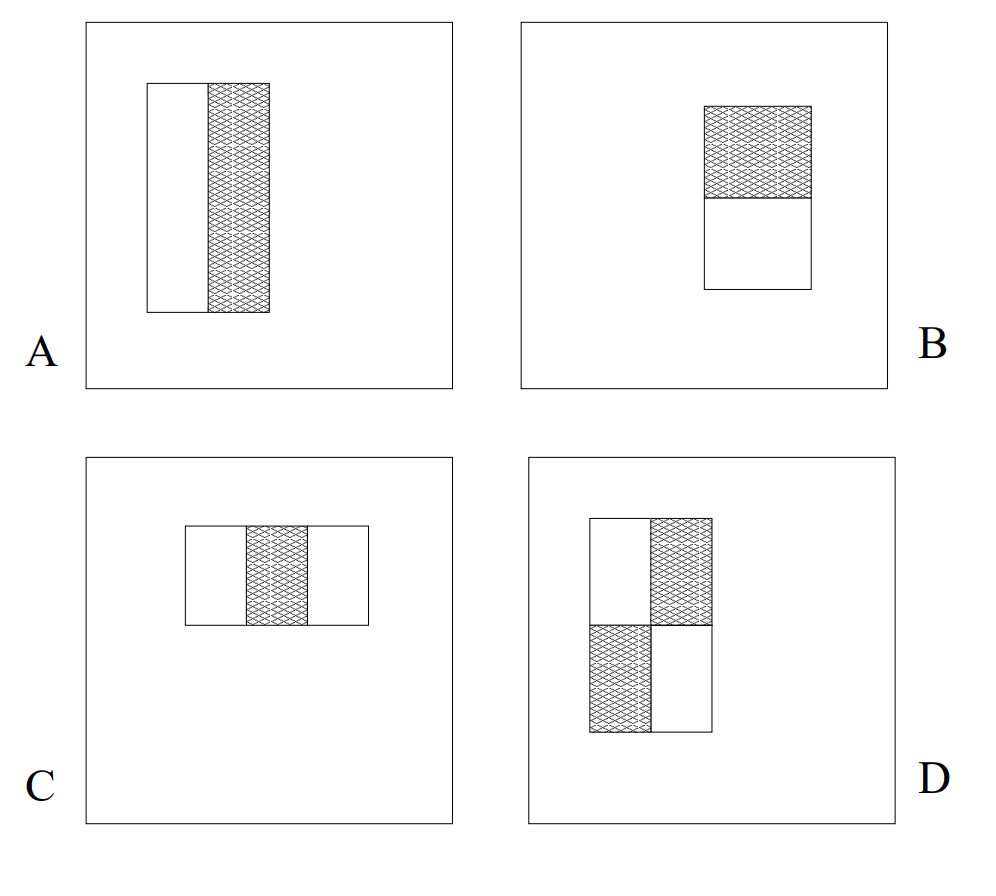
\includegraphics[width=0.7\textwidth]{Figures/haar1.png}
	\caption{Haar - dvoj-obdĺžnikové príznaky (A, B), troj-obdĺžnikové príznaky (C) a štvor-obdĺžnikové príznaky(D)\cite{viola2001robust}}
	\label{fig:Haar1}
\end{figure}

\begin{equation}
ii(x,y)=\sum_{x^{\prime}\leq x,y^{\prime}\leq y}i(x^{\prime},y^{\prime}),
\label{eq:Výpočet integrálneho obrazu}
\end{equation}


\newpage
\subsection{HOG}
\label{HOG}
S nápadom  vylepšiť detekciu objektov použitím príznakov prišli v roku 2005 Navneed Dalal a Bill Triggs \cite{dalal2005}, kde postupne vyskúšali niekoľko typov deskriptorov.  V práci taktiež podobne rozobrali  možnosti a spôsoby ako správne určiť parametre ich detekčnej metódy pre správne fungovanie detekcie jednotlivých tried. Podstatou ich metódy je, že objekt môže byť  charakterizovaný  viacerými spôsobmi. Táto metóda je rozdelená do niekoľkých samostatných krokov (Obr. \ref{fig:HOG1}):
\begin{itemize}
  \item \textbf{Úprava obrazu} - v tomto kroku je potrebné  v obraze upraviť konktrast a jas , ktoré by mohli spôsobovať  problémy v nasledujúcich krokoch. Okrem tejto úpravy  je možné  obraz urpaviť napríklad gamma filtrom.
  \item \textbf{Výpočet gradientov} - veľkosť gradientov sa počíta na základe vstupného obrazu a masky. Masky, ktoré sa používaju v tomto kroku sú \textit{[-1, 0, 1]} alebo \textit{[-1, 0, 1] \textsuperscript{T}}. Gradienty je nutné vypočítať v obidvoch osách, čím získame \textit{I\textsubscript{x}} a \textit{I\textsubscript{y}}. Po získaní gradientov je potrebné vypočítať veľkosť gradientov \textit{m(x,y)} a ich smer \textit{$\theta(x, y)$}.
  
  \begin{equation}
m(x,y)= \sqrt{I_{x}^{2} + I_{y}^{2}}
\label{eq:Výpočet veľkosti gradientu}
\end{equation}

  \begin{equation}
\theta(x, y) = \left(\frac{I_{y}}{I_{x}}\right)
\label{eq:Výpočet smeru gradientu}
\end{equation}
  \item \textbf{Normalizácia} -  Pre správne fungovanie je potrebné obraz normalizovať, aby sa minimalizovali rozdiely medzi jednotlivými bunkami. Tento krok spočíva v skladaní viacerých buniek, čím následne vznikajú bloky. 
   \item \textbf{Deskriptor} -  Je vytvorený zo vstupného obrazu do jednotlivých blokov. Jednotlivé bloky sa posúvajú a prekrývajú o daný počet pixelov. Výsledok desktiproru je odovzdaný  klasifikátoru, ktorý následne určuje do akej triedy objekt patrí. Jeden z často používaných klasifikátorov je Support vector machine (SVM), ktorý napríklad používali autori práce na efektívnu detekciu chodcov.\cite{pang2011efficient}
 \end{itemize}


\begin{figure}[ht]
	\centering
	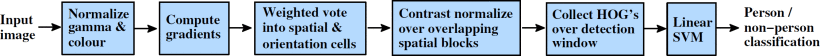
\includegraphics[width=1\textwidth]{Figures/hog.png}
	\caption{HOG - séria krokov \cite{dalal2005}}
	\label{fig:HOG1}
\end{figure}

\begin{figure}[ht]
	\centering
	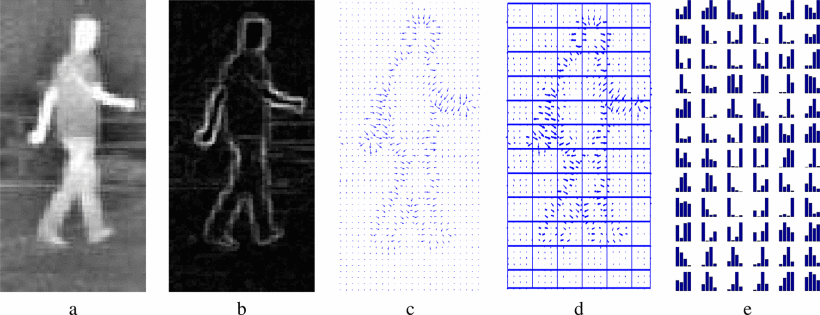
\includegraphics[width=0.8\textwidth]{Figures/hog3.png}
	\caption{HOG - vstupný obraz (a), normalizácia gradientu (b), orientácia gradientu (c), rozdelenie do buniek (d) vypočítaný histogram (e). \cite{bertozzi2007pedestrian}}
	\label{fig:HOG2}
\end{figure}


\newpage
\section{Detekcia pozície vodiča}
\label{sec:Pose detection}
Nieco  o detekciach pozicie


\newpage
\subsection{OpenPOSE}
openPose


\newpage
\subsection{TensorFlow}
tensorflow


\newpage
\subsection{Ostatné metódy}
WrnchAI





\newpage
\section{Využitie sférických kamier v automobiloch}
\label{sec:Spherical cameras}
Počas vypracovania diplomovej práce som mal zapožičané 2 sférické kamery. 

\subsection{Technické parametre}
Go PRO:

THETA:

Senzor	FishEye CMOS 2x12MPix
Maximálne rozlíšenie (Video)	4K  30fps
Maximálne rozlíšenie (Fotografia)	14.5MP (5376x2688px)
Svetelnosť	f2.0
Vnútorná pamäť	19GB


\begin{equation}
\left(\sum_{n=1}^{\infty}a_{n}b_{n}\right)^{2} \leq
\sum_{n=1}^{\infty}a_{n}^{2} \cdot \sum_{n=1}^{\infty}b_{n}^{2}
\label{eq:A}
\end{equation}



\newpage
\subsection{Použitie v analýze videa}
Problem s formatom videa, rozlisenim , deformaciou  hroe a dole



\newpage
\section{Program}
\label{sec:Program}
Zhrnutie vysledkov


\newpage
\subsection{Požiadavky a návrh programu}
Architekruta , schemy


\newpage
\subsection{Pozícia vodiča}


\newpage
\subsubsection{Detekcia}
NN klasifikator


\newpage
\subsubsection{Neurónová sieť}
NN klasifikator



\newpage
\subsection{Orientácia hlavy}


\newpage
\subsection{Výstup programu}
obrazky

\newpage
\subsection{Porovnanie výsledkov}
porovnanie


\newpage
\subsection{Využitie zozbieraných dát}
porovnanie


\newpage
\subsection{Používateľská príručka}
python program.py --use-openPose=true


\newpage
\section{Možnosti vylepšenia detekcie}
\label{sec:Možnosti vylepšenia detekcie}
Zhrnutie vysledkov


\newpage
\section{Záver}
\label{sec:Zaver}
Zhrnutie vysledkov







\bibliography{literatura}














\end{document}
